\section{Introduction}
In recent years, many industries have experienced enormous changes due to an influx of enormous quantities of data, a greater availability of data storage and high computational power, and an ever-increasing armoury of machine learning algorithms and methods. The aviation industry is no exception to this: the Airbus A350 XWB, for example, comes equipped with approximately \numprint{6000} sensors that produce 300 GB of data every day; the next generation Airbus A380 will come with \numprint{10000} sensors on a single wing alone \cite{rajaraman_big_2016}.

Modern airliners are reliant on a constant stream of \ac{ehm} data for monitoring the status of the aircraft during the flight. A post-flight review of the data and a subsequent adjustment of flight manoeuvres can offer significant improvements in fuel efficiency and minimise component fatigue. As an optional aftermarket service, Rolls-Royce offers Efficiency Management and Efficiency Optimisation, which use \ac{ehm} data with \textquote{cutting-edge technology such as machine learning and applied analytics} to optimise customers' use of their engines \cite{rolls-royce_plc_airlines_2020}.

The ability to process this data in a reliable and efficient way is paramount for carrying out these analyses. Using highly optimised, specially designed programming libraries, data-orientated machine learning approaches are more accessible and more powerful than ever, and can produce excellent results in detecting patterns in data and evaluating these accordingly. 

\subsection{The Engine}
The Civil Aerospace department of Rolls-Royce designs and manufactures primarily high-bypass turbofan jet engines, which offer an ideal arrangement for civil aircraft flying below the speed of sound \cite{rolls-royce_plc_jet_2015}.

Engines consist of four main components (fan, compressor, combustion chamber and turbine) which correspond approximately to the four stages of a Brayton cycle (intake, compression, combustion, expansion). The engine draws in air, compresses it, burns fuel in the compressed air and forces this air out through the rear nozzle, while extracting some energy at the turbine stage to continue powering the fan and compressor \cite{rolls-royce_plc_jet_2015}.

To increase thrust and efficiency, many modern civil aircraft engines are equipped with two concentric shafts, split into \ac{lp} and \ac{hp}, which connect respective sets of compressors and turbines \cite{spittle_gas_2003}. Some, including the Rolls-Royce Trent family of engines, also have a third shaft, coupling the \ac{ip} compressor and turbine. Figure \ref{fig:triple_spool} shows a rough configuration of such an engine. 

\begin{figure}
    \centering
    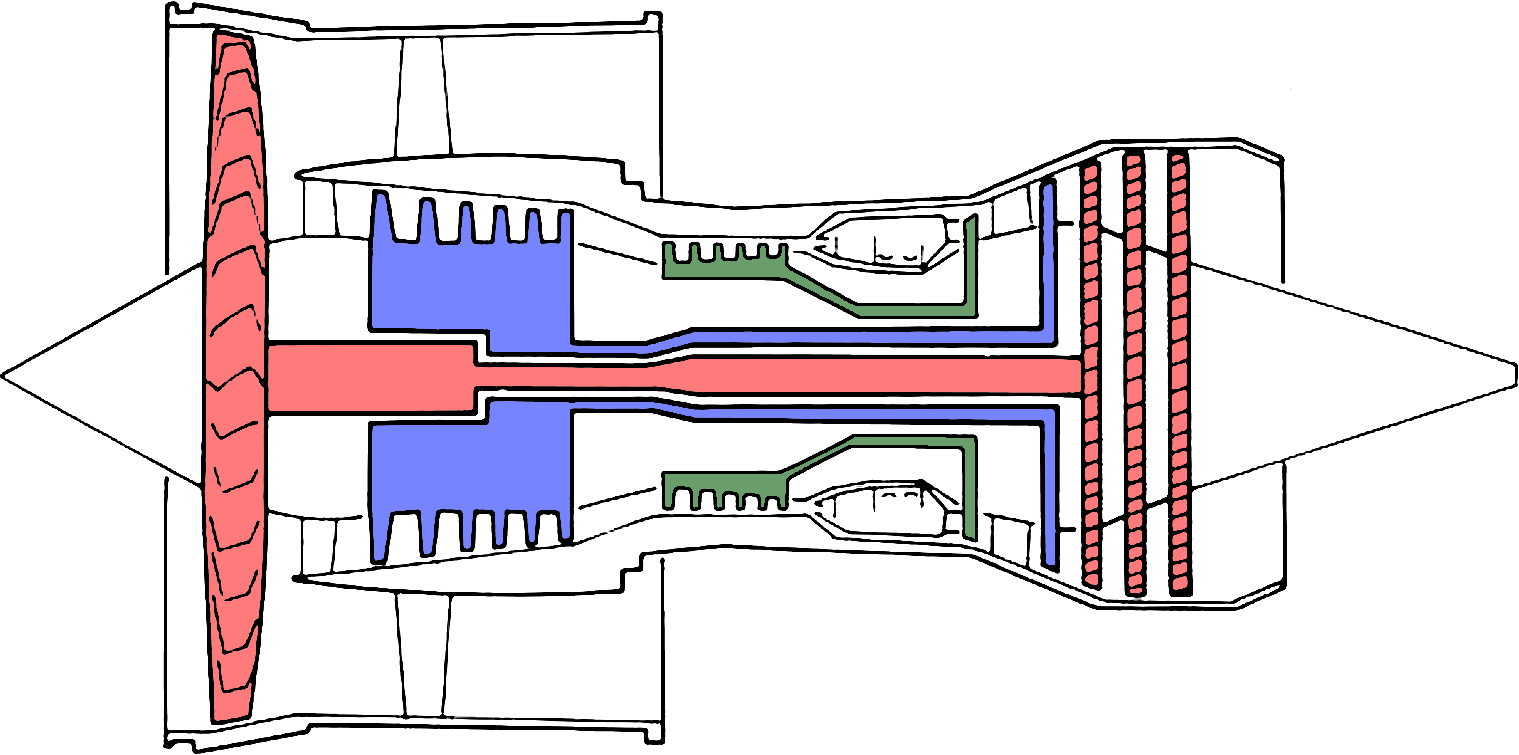
\includegraphics[width=0.7\textwidth]{triple_spool}
    \caption{\label{fig:triple_spool} A schematic diagram of a triple-spool high-bypass engine with \ac{lp}, \ac{ip} and \ac{hp} components shown in red, blue and green, respectively (based on \protect\cite{rolls-royce_plc_jet_2015}).}
\end{figure}


While this arrangement has greatly improved efficiency, it comes with the compromise of significantly increased temperatures within the engine, particularly as the air passes from the combustion chamber to the \ac{hpt}. The \ac{tet} has risen to such an extent that \ac{hpt} blades now operate in temperatures far above their melting point, requiring great improvements in the materials, structures and systems used, such as extracting cooler air from the compressor stage and releasing this through air holes in the blades to create an insulating barrier between the blade and hot air \cite{spittle_gas_2003}.

\subsection{Damage}
Components used in such extreme conditions experience degradation. They therefore cannot be used indefinitely and must be removed from service after a certain amount of time to avoid potentially catastrophic failure. The amount of time for which the component is permitted for service, referred to as its Approved Life, is determined in safety analyses \cite{easa_certification_2015}. Approved Life is measured in Engine Flight Cycles, to be referred to as \textit{cycles} in the following. (These aspects will be discussed in more detail in Section \ref{certif}.)

The degradation of the engine through its use is referred to as damage, whose unit is also cycles. The extent of damage is dependent on many parameters: Since operators use their aircraft for different purposes, flight parameters such as duration and altitude vary greatly and cause different levels of damage. 

In a \ac{fe} context, components are modelled digitally and separated into a finite number of individual elements, the corner points of which are called nodes. Areas of particular interest within the component (usually where stresses are expected to be highest) are referred to as features. 

Within Rolls-Royce, damage from flight missions is currently calculated using one of two internal tools for flight profile analysis: SA66 and Perseus (see Sections \ref{sa66} and \ref{pers}, respectively). The former is ideal for processing many flights in a short amount of time, but is restricted to a low number of features due to the time involved in manually setting up the surrogate \ac{fe} model for each feature. The latter can be described as a brute-force method that determines damage for all surface nodes, but is restricted by the amount of time required to process a single flight.

\subsection{Artificial Intelligence}
\ac{ai}, the field of research that occupies itself with giving machines the ability to think and learn, has been the focus of much research in recent years due to the increasing capabilities of hardware to tackle the challenges it involves, as well as its profitability in industries looking to implement automation of routine labour or optimise data analysis tasks \cite{goodfellow_deep_2016}.

One subfield of \ac{ai} is \ac{ml}, in which machines extract information and patterns from data without thorough or explicit instructions, usually making use of highly contrived data from which noise (non-critical background information) has been removed. Classifying objects based on a finite set of input values (e.g. birds based on their weight, wingspan, the colour of their back and whether they have webbed feet \cite{harrington_machine_2012}) is an ideal task for machine learning. 

\ac{ml} tasks are generally split into two categories: supervised and unsupervised learning \cite{kelleher_fundamentals_2015}. The former involves training the model to associate input data with known output data and using it on previously unseen data; in the latter, a model is given data and instructed to find patterns or groups based on input data alone \cite{goodfellow_deep_2016}.

\ac{dl} is an application of \ac{ml} that employs more complex models capable of making sense of noisier, largely unprocessed data, such as sound signals and images \cite{goodfellow_deep_2016}. Classifying birds could in this case involve extracting necessary information from an image or diagram of the bird, requiring far less manual measurement or input.

\ac{dl} has seen a huge rise in popularity in recent years, with applications including speech recognition \cite{deng_machine_2013}, medical diagnoses \cite{lee_diagnosis_2018}, stock market prediction \cite{krollner_financial_2010} and many others \cite{kelleher_fundamentals_2015}. One particular challenge among the \ac{dl} research community is time series data \cite{yang_10_2006}, a sequential collection of values recorded over time. Time series data remains a great challenge due to its noisy, multidimensional nature \cite{kelleher_fundamentals_2015} and the dfficulties involved in developing algorithms that can also interpret the temporal information held in the signal \cite{bagnall_great_2017}. 

\subsection{Motivation}
It is in the interest of Rolls-Royce to improve the speed and accuracy of \ac{ehm} data analysis to gain an overview of the performance and remaining Approved Life of in-service engines. 

The goal of the present thesis is therefore to identify a supervised machine learning approach that offers a robust, verifiable, comprehensive, fast and sufficiently accurate means of processing \ac{ehm} data to determine the extent of damage incurred by surface nodes of a component during real flight missions. 